Below are the list of methods we will be using to solve the project goals.

\begin{itemize}

\item \textbf{Graph Representation}
\bigskip
In order to be able to predict the atomic scale fracture nucleation and propagation in silica-based glasses, we must first find an appropriate mathematical graph representation. 
\begin{itemize}
    \item \textbf{Basic Graph Representation}
    \\
    The most basic way to define a graph is naive. In one sample, we have a total number of $n$ atoms. An atom, either a Silicon atom or an Oxygen atom, is defined as a vertex $v_i$, where $0 \leq i \leq n$ and a set of such vertices is $\mathbf{V} = \{v_0,v_1,...v_{n-1}\}$. An edge, $e_i$ is defined as a mechanical trusses between two atoms. A set of such edges is $\mathbf{E} = \{e_0,e_1,...e_{n-1}\}$. As uni-axial stress is applied to the material, edges could break and form between any two vertices, where state 1 means an edge is broken and state 0 means an edge exists. Therefore, an set of active edges, defined as $\mathbf{E_a}$, includes all the edges that have broke or formed at least once, meaning they have changed their state, either from 1 to 0 or from 0 to 1 at one point. As a result, the graph \textbf{G} is thus defined as a discrete set of vertices \textit{V} connected by a set of edges \textit{E}. We can denote it as $\ G = (V,E)$, where the size of the graph is $\ |V| = n $.
    
    \item \textbf{Reduced Graph Representation}
    \\
    
    
\end{itemize}


\item \textbf{Feature Description}
\bigskip

To use ML algorithms, we want to characterize vertices based on features such as charge, stress tensor, type and centrality.

\begin{itemize}
    \item \textbf{Centrality:} In graph theory, centrality is use to identify the most important vertices. An example could be a specific silicon atom that is at the center of where a fracture nucleates. Identifying these vertices with the most centrality will allow us to predict fracture
\end{itemize}







\\

\item \textbf{Machine Learning Methods}
\bigskip
\\


\textit{Below are old stuff}
\item \textbf{Method for Identifying Fracture Nucleation} 
\bigskip
\\

Lets construct our own simple graph. 
\bigskip
\\
% CONSTRUCTION OF EXAMPLE GRAPH SiO3 %%%%%%%%%%%%%%%%%%%%%%%%%%%%%%%%%%%%%%%%%%%%%%%%%%%%%%%%%%%%%%%%%%%%
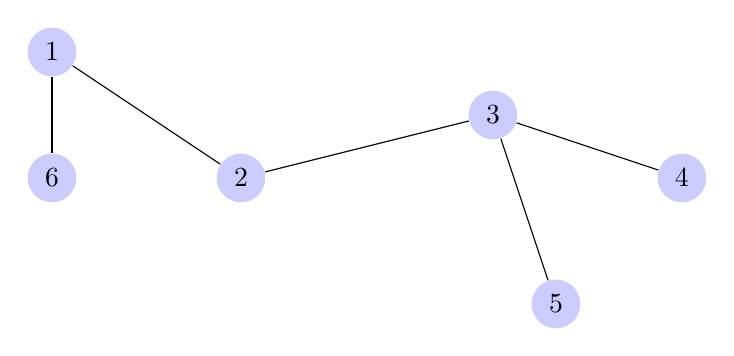
\begin{tikzpicture}
  [scale=.8,auto=left,every node/.style={circle,fill=blue!20}]
  \node (n6) at (1,10) {1};
  \node (n4) at (4,8)  {2};
  \node (n5) at (8,9)  {3};
  \node (n1) at (11,8) {4};
  \node (n2) at (9,6)  {5};
  \node (n7) at (1,8)  {6};

  \foreach \from/\to in {n6/n4,n4/n5,n5/n1,n2/n5,n6/n7}
    \draw (\from) -- (\to);

\end{tikzpicture}
%%%%%%%%%%%%%%%%%%%%%%%%%%%%%%%%%%%%%%%%%%%%%%%%%%%%%%%%%%%%%%%%%%%%%%%%%%%%%%%%%%%%%%%%%%%%%%%%%%%%%%%%%%
\bigskip
\\
% THIS IS PRETTY WONKY NOTATION MAYBE A BETTER WAY OF LABLING ??

Since we will be working with a large data set of vertices, we can store degree information for each vertex in a \textbf{degree matrix}. Given a graph $\ G(V,E)$ where \textit{n} is the number of nodes, the degree matrix of G is a diagonal matrix who's entries are the degree of each vertex. 
\bigskip
\\


For our project, creating the graph representation as a fracture system may present difficulties. The reason for this being that as stresses are added to the silicate glass, the size and location of a fracture changes over time, forcing the node to also change and making the system a more dynamic process.
\bigskip
\\
\\
With this being said, we want to fix number of nodes at the initial start time, and for this value to remain constant throughout the fracture propagation. We do this in order to keep track of whether or not fractures combine together.
\bigskip
\\
\\
Therefore, we can perhaps define nodes as a single atom, Si or O. Doing this to our constructed graph could result like this:
\bigskip
\\
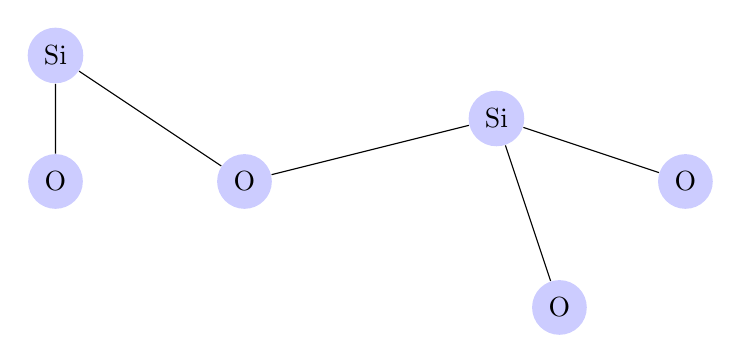
\begin{tikzpicture}
  [scale=.8,auto=left,every node/.style={circle,fill=blue!20}]
  \node (n6) at (1,10) {Si};
  \node (n4) at (4,8)  {O};
  \node (n5) at (8,9)  {Si};
  \node (n1) at (11,8) {O};
  \node (n2) at (9,6)  {O};
  \node (n7) at (1,8)  {O};

  \foreach \from/\to in {n6/n4,n4/n5,n5/n1,n2/n5,n6/n7}
    \draw (\from) -- (\to);

\end{tikzpicture}
\bigskip
\\
Due to the rapid nature of change within the molecular dyanmic simulations, there is one problem that must be address. The exploration of a single graph, or multi graph representation. This will be a challenge that we will have to investigate.   

\item \textbf{Method for Identifying Local Structures in the Graph}
\bigskip
\\
In order to predict where a fracture nucleates we must be able to identify any structures within the graph that might be associated with a fracture. Our above graph as we said was undirected and unweighted but if we look closer we can see associated structures. There are two molecules present in the graph, an $\ SiO_{3}$ and an $\ SiO_{2}$. Together they both share 1 oxygen atom, this is called a \textit{covalent} bond.
\bigskip
\\
Glasses containing nano-voids and atomic defects (such as under- and over-coordinated silicon and oxygen atoms) are less brittle than flaw-free bulk glasses. As fractures occur and propagate, there are more under- and over-coordinated silicon and oxygen atoms. We want to utilize this information as we utilize our adjacency matrix in our prediction on nucleation events. 
    \item \textbf{Stress Tensors:} We want to consider the direction in which the stress tensor is being applied. This has a direct affect on the size of a fracture and where it will emerge.
\end{itemize}

\begin{itemize} \item \textbf{Feature Extraction} 
\bigskip
\\
We plan to identify features of the graph network by using machine learning (ML) techniques. We aim to construct a ML algorithm that we will use to train data. This data is represented at time steps and will enable us to make predictions of where fractures will occur for later time steps. We will construct this graph using adjacency matrices.

To find features, we want to examine the relationship between nodes and fractures, which we may do so using the radial distribution function (RDF) or the k-nearest neighbors algorithm (KNN). Doing so will allow us to identify the smallest distance nodes may be within one anther before a fracture emerges.
\bigskip
\\
\textbf{Radial Distribution Function:} The radial distribution function (RDF) measures the probability of a node existing at a given distance away from a specific particle. To construct this function we pick a node and draw a series of concentric circles around it at a fixed distance. The number of atoms found in each shell is counted and stored at periodic intervals. The average number of atoms in each shell is calculated at the end of the simulation. To get the RDF, that average is then divided by the volume of each shell and the average density of the atoms. We will use the RDF to examine node distance periodically throughout the simulations, specifically when fractures begin. The RDF is also known as a radial pair distribution function. We can use the Average Radial Distribution function or the site-specific radial distribution function. The former calculates between two groups of atoms while the latter takes as input a list of pairs of atomic groups and outputs a list of RDF's between specific atomic groups.
\bigskip
\\
\textbf{K-nearest Neighbor:} The K-nearest neighbor (KNN) classification can help us predict the borders of the fractures. We can pick a random node and implement the KNN. We can classify that node either as that it contributed to the fracture or it didn't contribute to the fracture. If the nodes are a certain distance away from each other, and a fracture exists, we would classify those nodes as having contributed to the fracture. The distance away that is required to contribute to the fracture is to be determined.
    

First, we plan to use the above extracted features to predict fracture nucleation from a initial structure with no fracture. Additionally, we want to examine damage, meaning how a fracture may lead to another fracture, and so on. In particular, can cracks be isolated and not contribute to any further damage? We aim to address this concern and more. Moreover, we want to implement alpha shape in order to analyze fracture orientation, then we will examine fracture velocity and fracture tips.

By examining these two features, we will be able to predict where an initial fracture may occur. We will then study the properties of this fracture to predict the future behavior of our structure.

To identify local structure, the 2017-2018 paper uses a Gaussian kernel to "convert distances to similarities" (page 5). Use this possibly? This paper also lists all the parameters and what they define the parameters to be.
\end{itemize}

\begin{itemize}
\item \textbf{Machine Learning Methods} 

The culminating purpose of this project is to produce a machine learning model based on supervised learning techniques. 


\end{itemize}

